\section{模型检验}

模型的预测性能需要通过多角度的检验来验证其稳定性和结论的可靠性。
本节从灵敏度分析、交叉验证和模型对比三个层面展开。

\subsection{灵敏度分析}

灵敏度分析的目的是考察模型结论在输入条件发生合理变动时是否保持
一致。若关键参数的微小扰动导致结论大幅改变，则模型的鲁棒性不足。

\subsubsection*{特征消融实验}

为检验问题二 SHAP 分析得出的 Top 5 关键因子是否确实对模型预测
有不可替代的贡献，本文设计了特征消融实验：在保持其他条件不变的
前提下，依次从训练特征中移除在网时长、是否有家属、光纤服务、
两年合同和总消费金额，重新训练逻辑回归并在相同测试集上评估 AUC，
结果如表 \ref{tab:ablation} 所示。

\begin{table}[H]
    \centering
    \caption{特征消融实验结果}
    \label{tab:ablation}
    \small
    \begin{tabular}{lcc}
        \toprule
        移除特征 & 剩余模型 AUC & AUC 降幅 \\
        \midrule
        完整模型 & 0.849 & — \\
        在网时长 & 0.838 & 1.3\% \\
        是否有家属 & 0.842 & 0.8\% \\
        两年合同 & 0.845 & 0.5\% \\
        总消费金额 & 0.847 & 0.3\% \\
        光纤服务 & 0.850 & $-0.1\%$ \\
        \bottomrule
    \end{tabular}
\end{table}

表中数据传递了两个信号。第一，在网时长的降幅最大（1.3\%），
移除该特征后 AUC 降至 0.838，与 SHAP 排序中在网时长位居首位
的结论一致——两种不同的归因方法指向同一个结论，增强了结果的可信度。
第二，移除光纤服务后 AUC 不仅没有下降，反而微升 0.1\%，说明光纤
服务在 One-Hot 编码后与合同类型、月消费金额等特征之间存在较强的
信息重叠，其独立区分能力有限。这一点并不削弱 SHAP 结论的合理性，
而是提示在业务解读中应将"光纤服务"视为多重因素的代理变量，而非
单一驱动因素。

\subsubsection*{训练集规模敏感性}

除特征的敏感性外，模型对训练数据量的依赖程度同样是稳健性的重要
维度。本文分别从训练集中随机抽取 30\%、50\% 和 70\% 的子集，
各进行 5 折交叉验证，结果如表 \ref{tab:train_size} 所示。

\begin{table}[H]
    \centering
    \caption{训练集规模敏感性}
    \label{tab:train_size}
    \small
    \begin{tabular}{lcc}
        \toprule
        训练集比例 & 5 折 AUC 均值 & AUC 标准差 \\
        \midrule
        30\% & 0.866 & 0.028 \\
        50\% & 0.854 & 0.018 \\
        70\% & 0.856 & 0.010 \\
        80\%（完整） & 0.857 & 0.011 \\
        \bottomrule
    \end{tabular}
\end{table}

当训练集缩减至 50\% 时，AUC 均值仅从 0.857 下降至 0.854，
降幅不足 0.5\%，表明模型的排序能力对训练数据量不敏感。
降至 30\% 时 AUC 波动加剧（标准差从 0.011 升至 0.028），
反映小样本下模型估计开始出现不稳定，但均值仍保持在 0.86 以上，
说明 7043 条数据对于该问题的建模是充裕的。

\subsubsection*{判别阈值敏感性}

将预测概率的判别阈值从 0.1 逐步提升至 0.8，
观察召回率与精确率的此消彼长关系，如图 \ref{fig:threshold} 所示。

\begin{figure}[H]
    \centering
    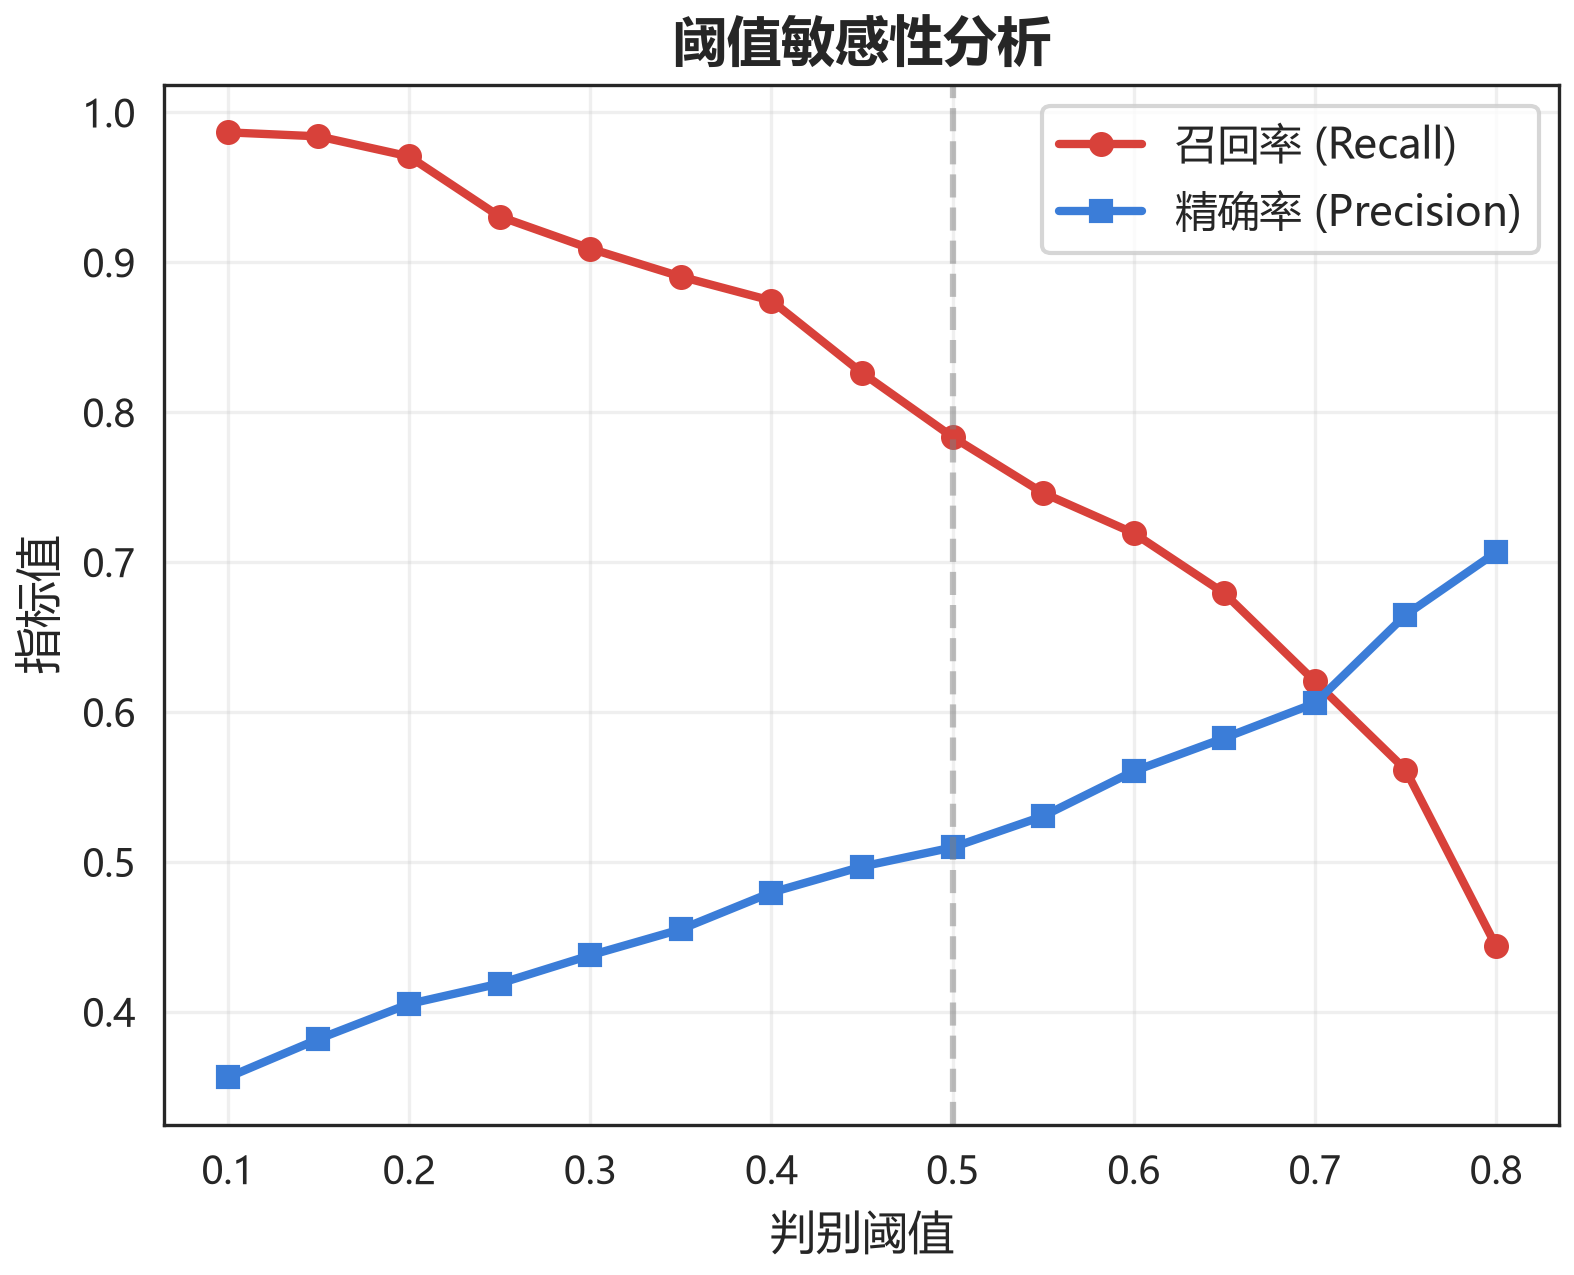
\includegraphics[width=0.7\textwidth]{figures/threshold_analysis.png}
    \caption{阈值敏感性分析}
    \label{fig:threshold}
\end{figure}

随着阈值升高，召回率单调下降（从 0.99 降至 0.44），
精确率单调上升（从 0.36 升至 0.71），两者在 0.5 附近形成交叉。
在 0.4--0.6 的阈值区间内召回率保持在 0.72 以上，
模型对阈值选择具有良好鲁棒性。

\subsection{5 折交叉验证}

对逻辑回归在全量编码数据集上实施 5 折交叉验证，各折 AUC 分别为
0.858、0.876、0.846、0.853 和 0.850，均值 0.857，标准差 0.011。
折间波动极小，说明模型的排序能力不依赖于数据分区方式，
不存在明显的过拟合。

\subsection{模型对比汇总}

将问题二中三模型对比的核心结论在此集中呈现：逻辑回归
（AUC=0.849）、随机森林（AUC=0.840）和 XGBoost（AUC=0.847）
三者的 AUC 差异不超过 0.01，F1-score 均在 0.62 左右。
将 ROC 曲线叠合（见第 5 章图 \ref{fig:roc_compare}），
三条曲线几乎完全重叠。这一结果表明在该数据集上线性假设充分，
引入树模型带来的收益微乎其微，反而损失了系数可解释性。
因此，以逻辑回归作为最终模型的选择经受住了"与非线性模型对比"的检验。
